\documentclass[10.5pt]{config}
% 本实验报告采用 署名-相同方式共享 4.0 国际许可协议 (CC BY-SA 4.0)
\usepackage{bigstrut,multirow,rotating,booktabs,makecell,array}%表格插件
\usepackage{color, xcolor}

\major{电子科学与技术}
\name{郑智瑄}
\partner{魏希浩} % 签名栏
% \title{}
\stuid{3230103913}
\date{\today}
\lab{东4-216}
\course{电子电路设计实验Ⅱ}
\instructor{叶险峰/施红军/邓靖靖}
\grades{}
\expname{实验设计报告} % 实验名字
\exptype{设计型} % 实验类型

\begin{document}

% \maketitlepage % 封面
% \maketoc % 目录
\makeheader % 首页头部

\section{设计项目实验结果与总结}
\subsection{实验目的}
设计电流-电压转换电路，将 4到20mA 标准电流信号转换为 
0到10V 的标准电压信号
\subsection{实验设计}
\subsubsection{原理图}
\begin{figure}[H]
    \centering
    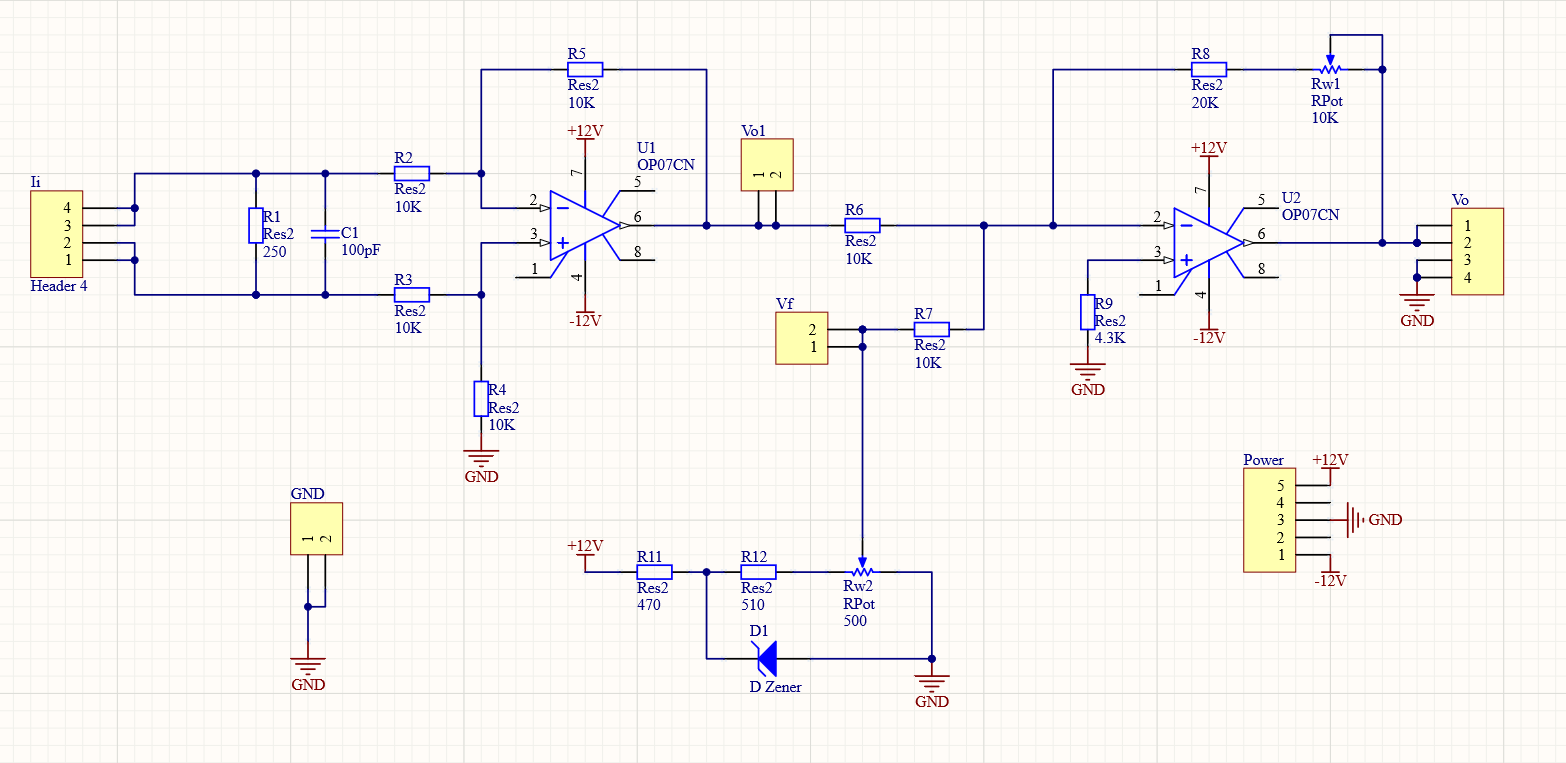
\includegraphics[width=0.55\textwidth]{figures/p01.png}
    \caption{示例项目原理图}
\end{figure}
\subsubsection{PCB图}
\begin{figure}[H]
    \centering
    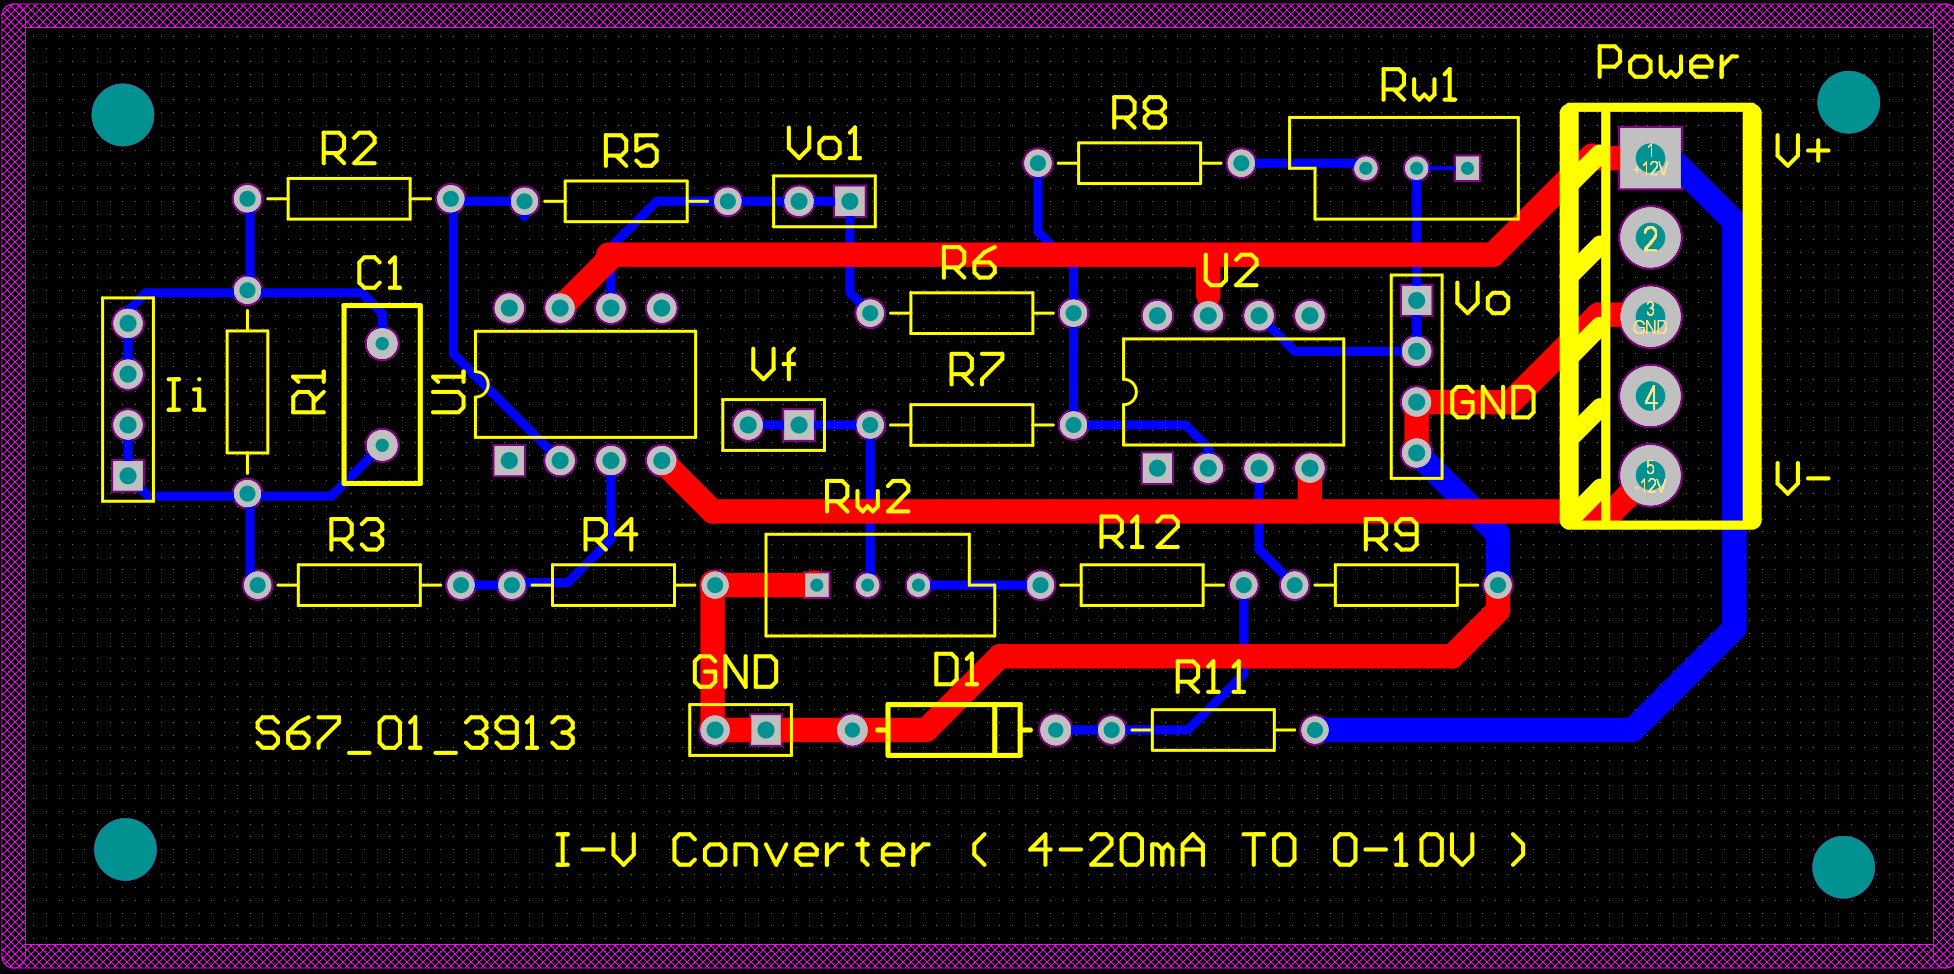
\includegraphics[width=0.55\textwidth]{figures/p02.png}
    \caption{示例项目PCB图}
\end{figure}
\subsection{实验结果}
\begin{figure}[H]
    \centering
    \subcaptionbox{测量结果1}[0.33\textwidth][c]{
        \centering
        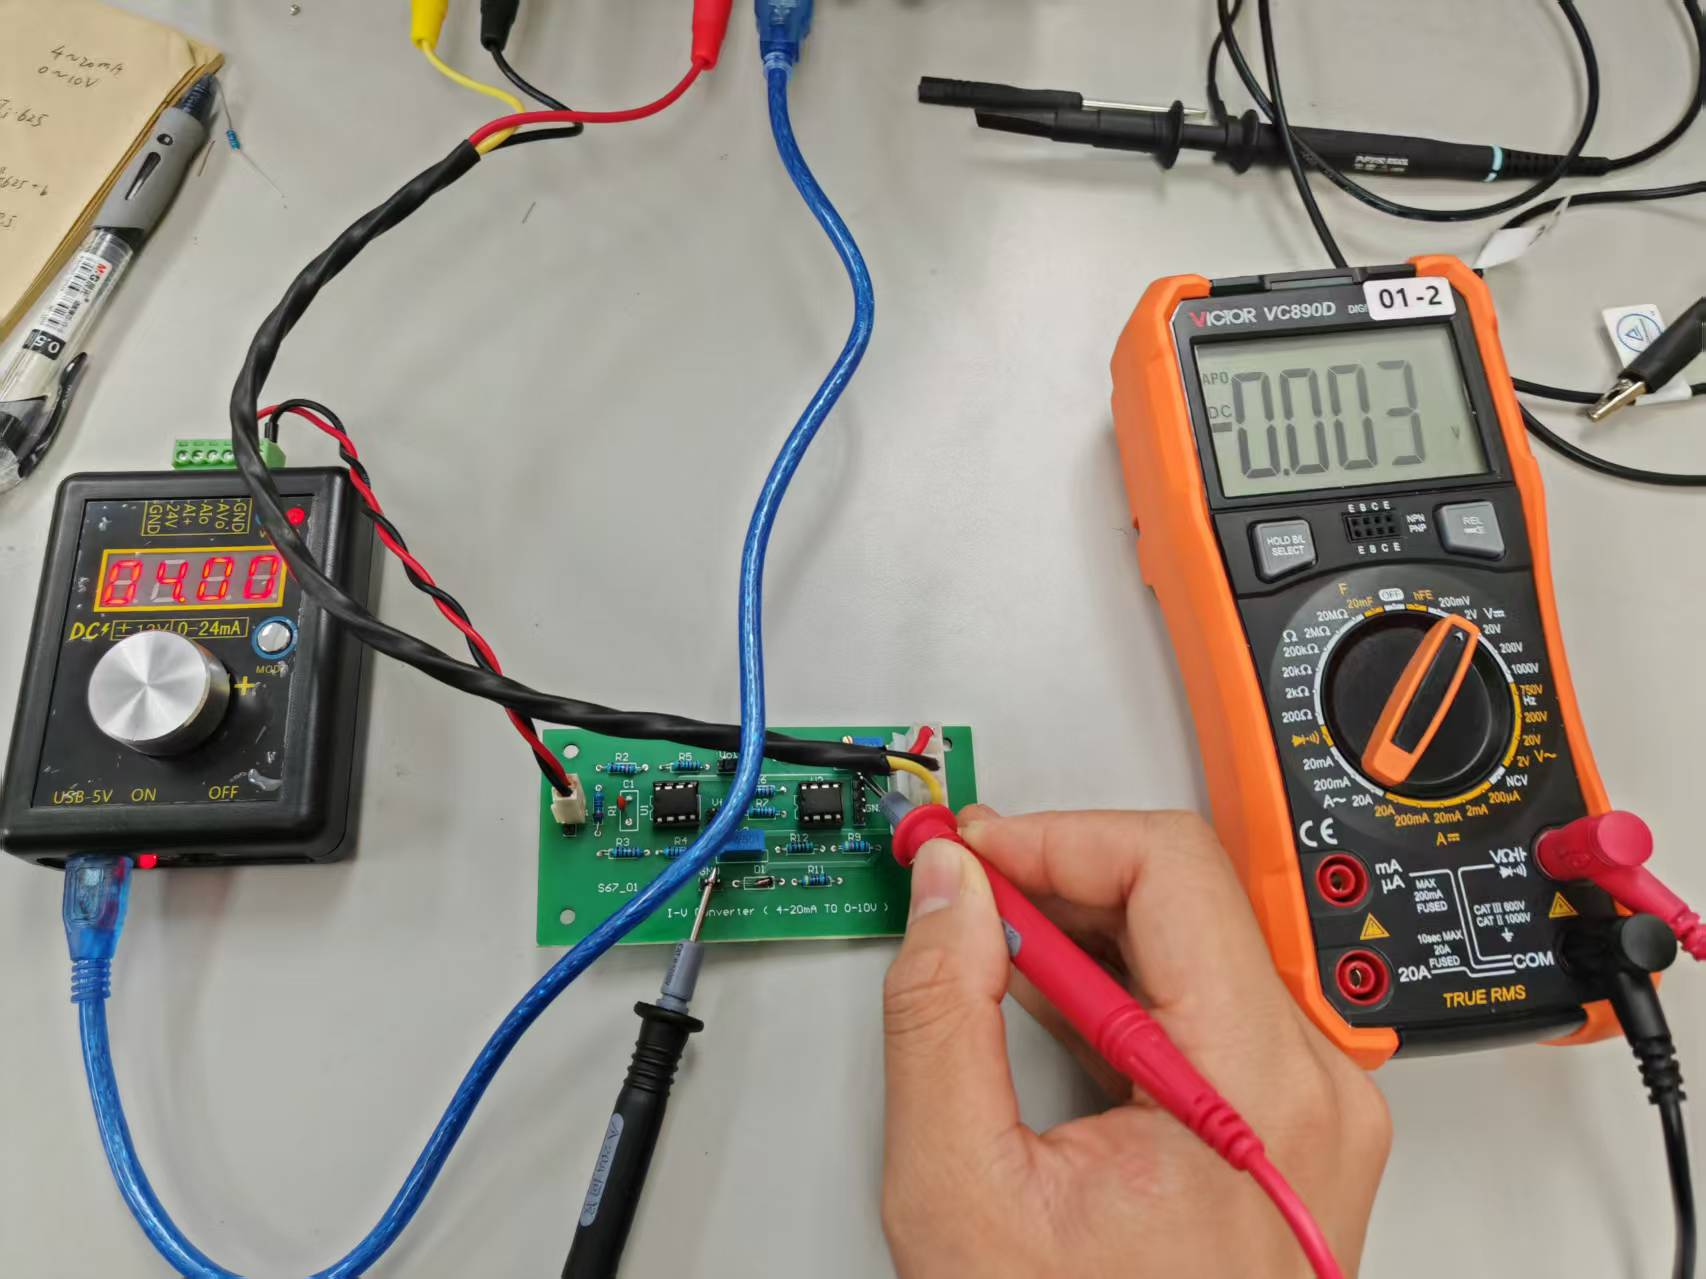
\includegraphics[width=0.32\textwidth]{figures/test1.jpg}
        \label{}
    }%
        \subcaptionbox{测量结果2}[0.33\textwidth][c]{
        \centering
        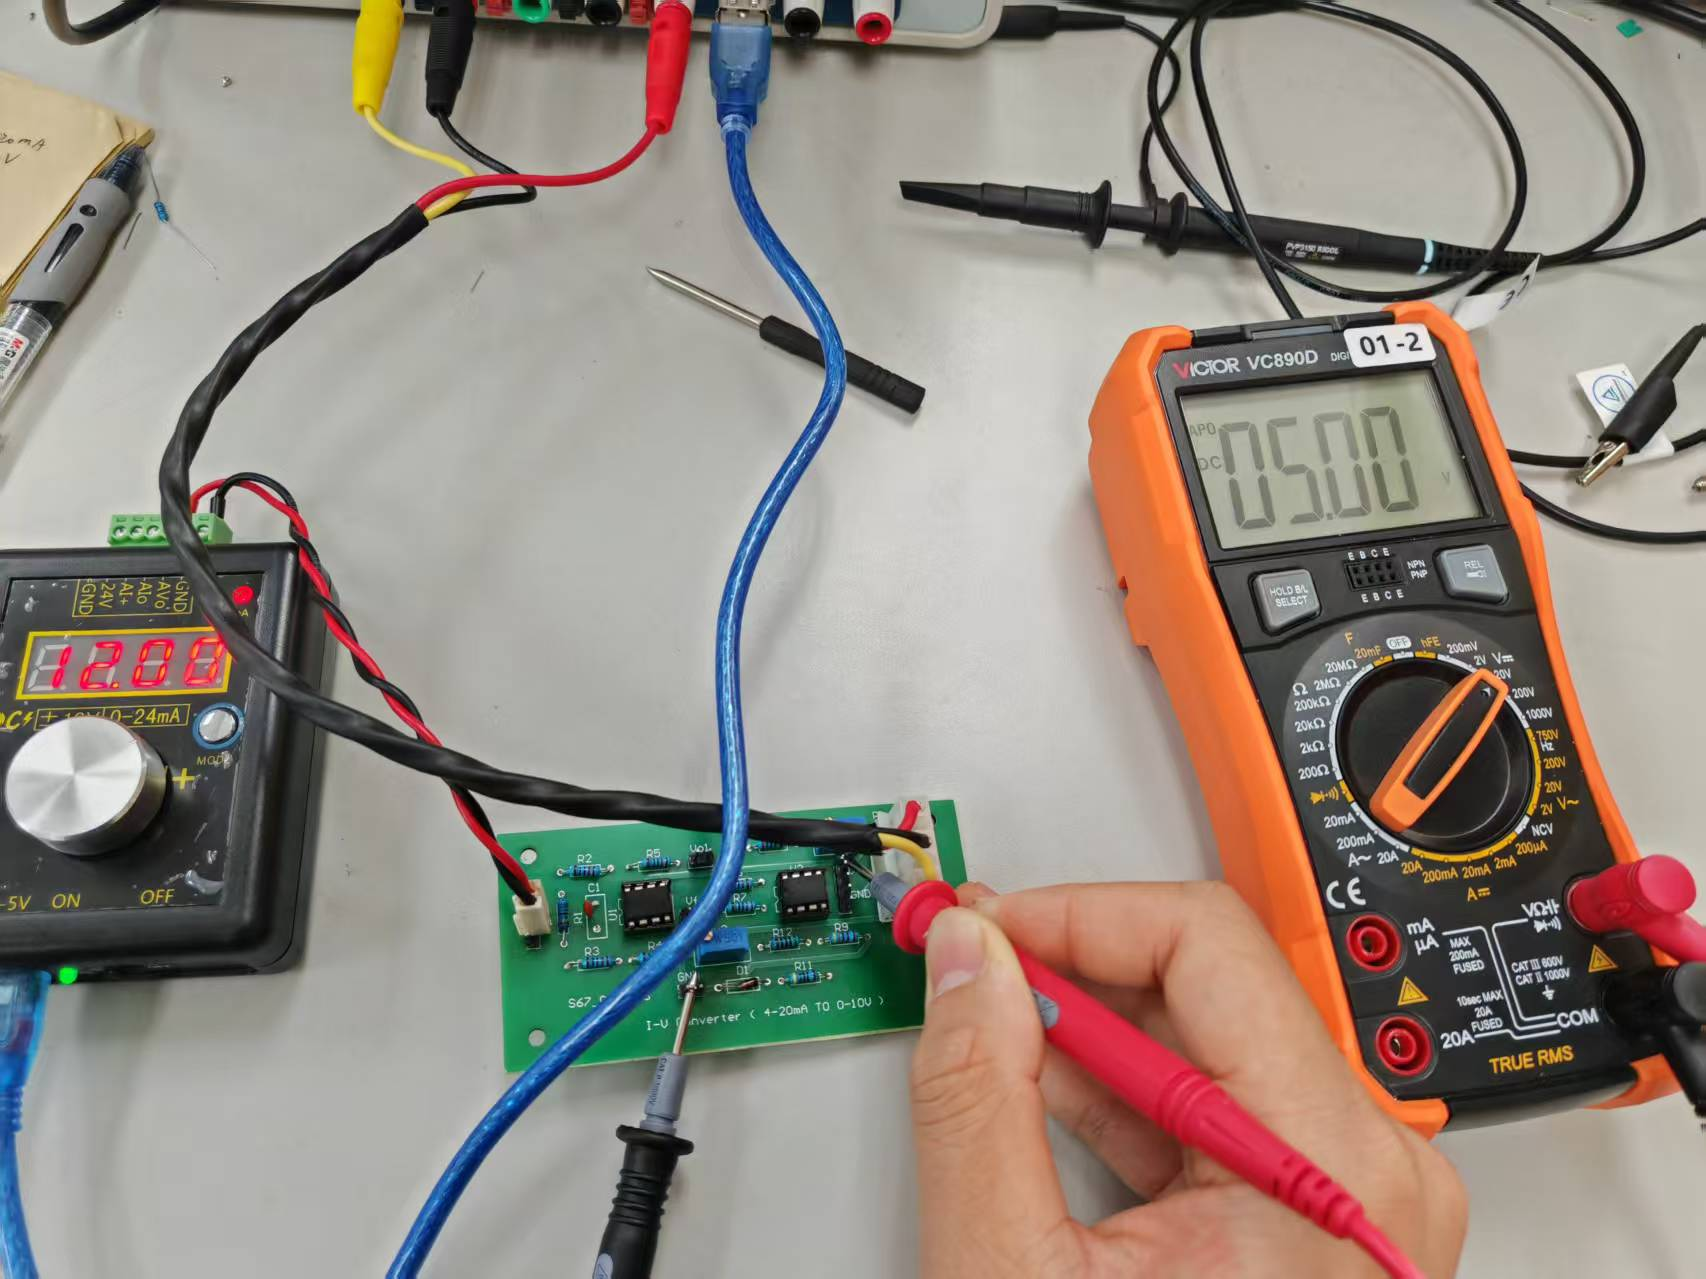
\includegraphics[width=0.32\textwidth]{figures/test2.jpg}
        \label{}
    }%
        \subcaptionbox{测量结果3}[0.33\textwidth][c]{
        \centering
        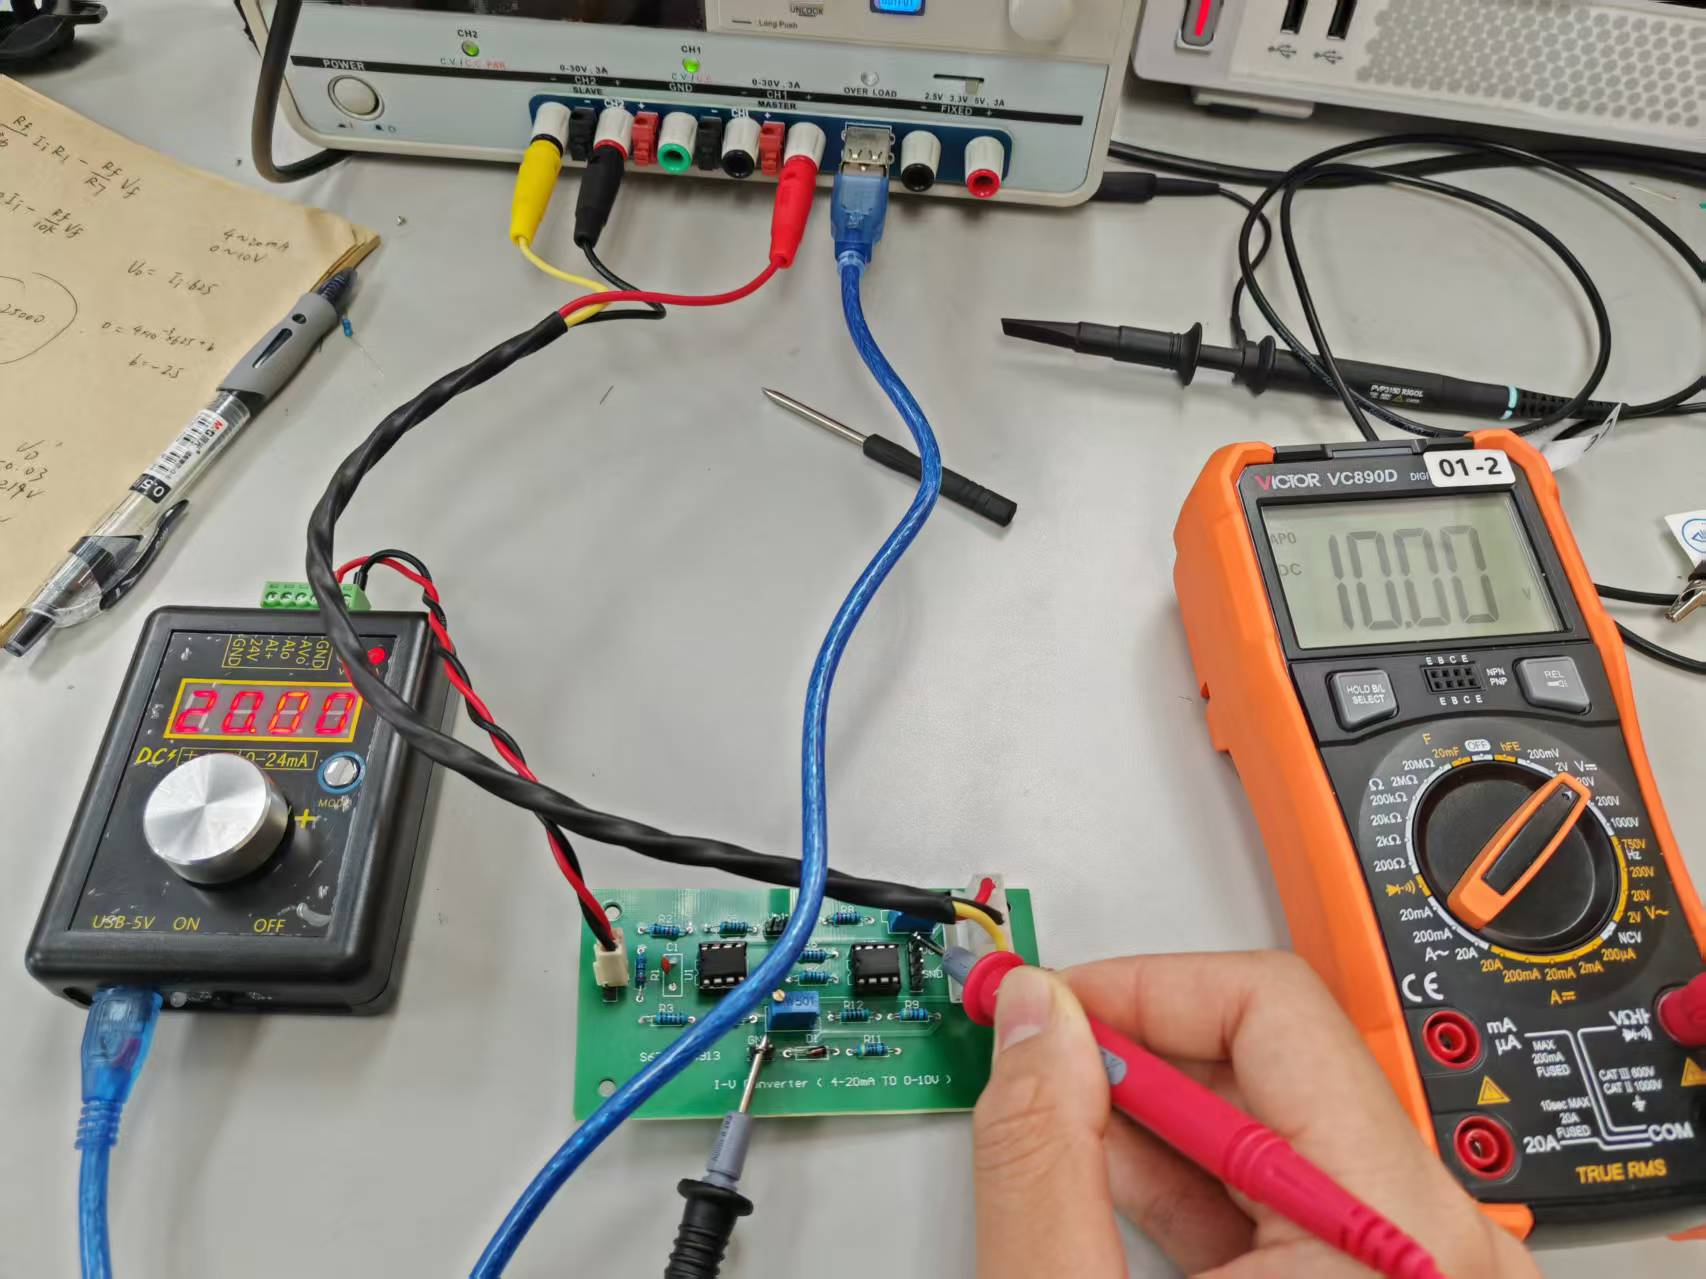
\includegraphics[width=0.32\textwidth]{figures/test3.jpg}
        \label{}
    }%
    \caption{测量结果图片}
    \label{}
\end{figure}
% Table generated by Excel2LaTeX from sheet 'Sheet1'
\begin{table}[H]
    \centering
  
      \begin{tabular}{|c|c|c|c|}
      \hline
      输入电流（mA） & 输出电压（V） & 理论值（V） & 相对误差（\%） \bigstrut\\
      \hline
      4.00     & -0.003 & 0     &  \bigstrut\\
      \hline
      6.00     & 1.246 & 1.25  & 0.32 \bigstrut\\
      \hline
      8.00     & 2.49  & 2.5   & 0.4 \bigstrut\\
      \hline
      10.00    & 3.74  & 3.75  & 0.27 \bigstrut\\
      \hline
      12.00    & 5.00     & 5     & 0 \bigstrut\\
      \hline
      14.00    & 6.25  & 6.25  & 0 \bigstrut\\
      \hline
      16.00    & 7.50   & 7.5   & 0 \bigstrut\\
      \hline
      18.00    & 8.75  & 8.75  & 0 \bigstrut\\
      \hline
      20.00    & 10.00    & 10    & 0 \bigstrut\\
      \hline
      \end{tabular}%
      \caption{测试结果表格}
    \label{tab:addlabel}%
  \end{table}%

  \begin{figure}[!htbp]
    \centering
    \begin{minipage}[b]{0.5\linewidth}
        \centering
        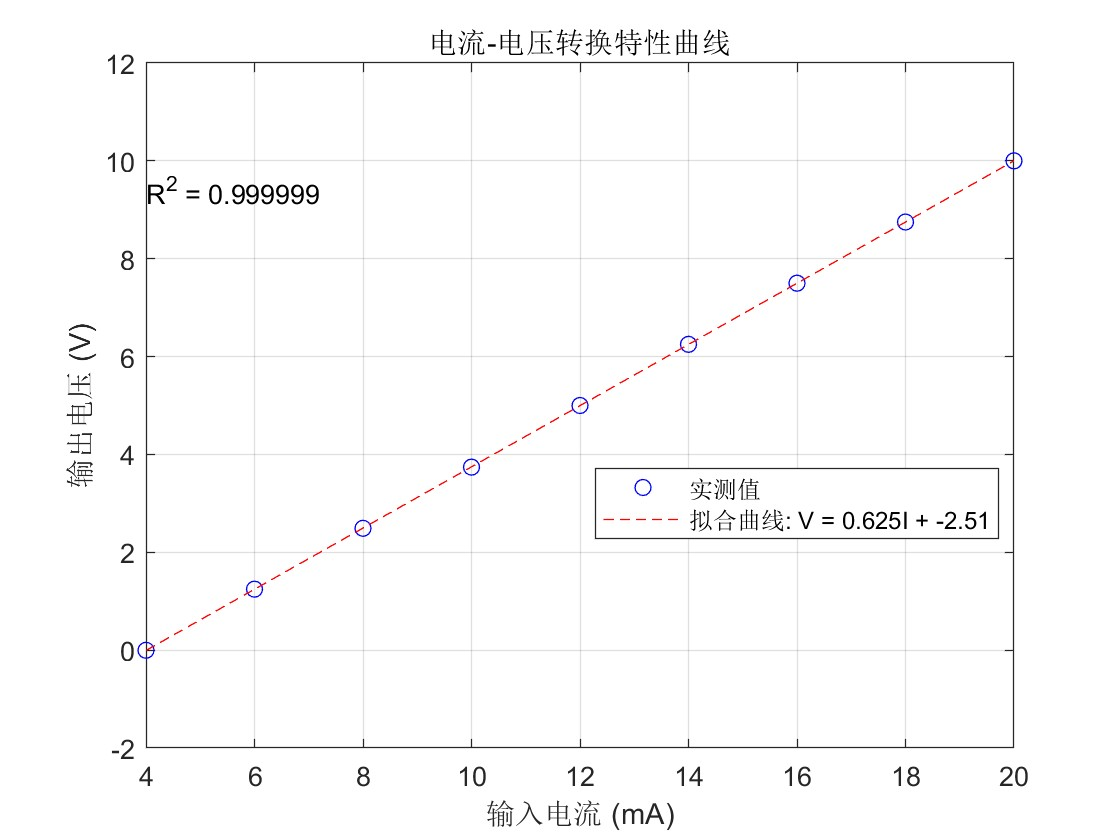
\includegraphics[width=0.9\textwidth]{figures/p02.jpg}
        \caption{电流-电压转换特性曲线}
        \label{}
    \end{minipage}%
    \begin{minipage}[b]{0.5\linewidth}
        \centering
        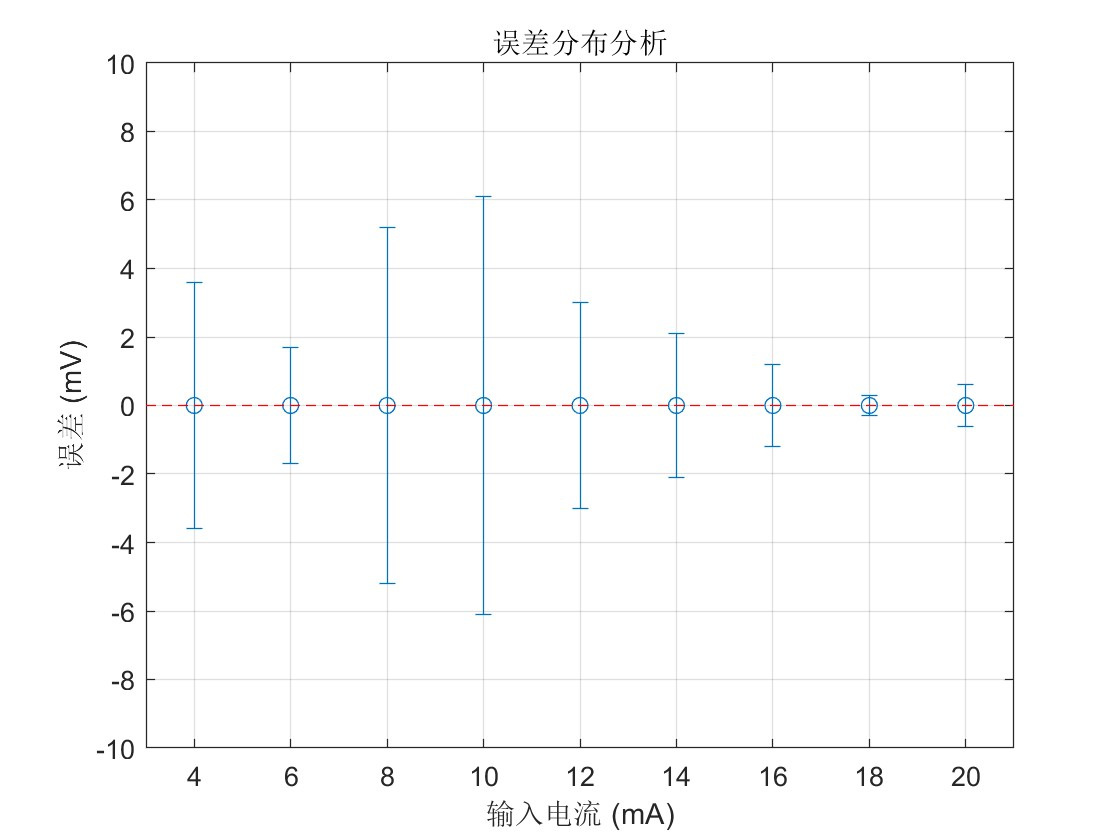
\includegraphics[width=0.9\textwidth]{figures/p03.jpg}
        \caption{误差分布分析}
        \label{}
    \end{minipage}
\end{figure}

【实验结论】：总体测试结果较为精确，拟合结果较好

\subsection{实验总结}
此次示例项目实践让我对电路设计的总体流程有了一个整体了解，从原理图设计，PCB设计与制作，PCB焊接到PCB调试，
也学会了软件Altium Designer的使用，对设计过程的一些坑如引脚配置，正负反接有了一定了解，能在之后去注意并且避免
\clearpage
\section{实验目的}
\begin{enumerate}[leftmargin=2em]
    \item 学习掌握用 Arduino UNO 设计数字时钟;
    \item 学习掌握PCB电路板的设计和制作;
    \item 学习掌握 Arduino UNO 扩展板的设计与制作;
    \item 学习掌握 DS1302 时钟芯片和 LCD1602 液晶显示屏的使用。
\end{enumerate}

\section{实验设计方案}
本项目使用 Arduino UNO 设计多功能数字时钟。硬件框图如Figure 1所示，下面对各部分模块进行说明。
\begin{figure}[!htbp]
    \centering
    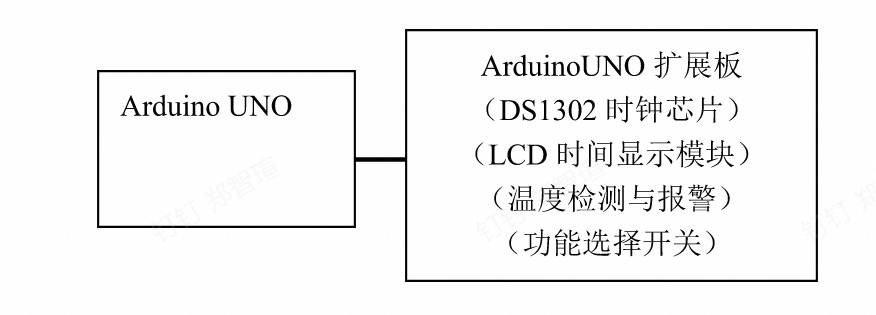
\includegraphics[width=0.8\textwidth]{figures/p1.png}
    \caption{多功能数字时钟框图}
\end{figure}

\textbf{DS1302 时钟芯片}

DS1302 是美国 DALLAS 公司推出的一种高性能、低功耗的实时时钟芯片，附加 31 字节静态 RAM，采用 SPI 三线接口与 CPU 进行同步通信，并可采用突发方式一次传送多个字节的时钟信号和 RAM 数据。实时时钟可提供秒、分、时、日、星期、月和年，一个月小与31 天时可以自动调整，且具有闰年补偿功能。工作电压宽达 2.5～5.5V。采用双电源供电（主电源和备用电源），可设置备用电源充电方式，提供了对后背电源进行涓细电流充电的能力。详细内容，可查阅芯片的 Datasheet。

\textbf{LCD 显示模块}

本次实验使用 Arduino UNO 直接驱动 1602 液晶显示字母和数字，LCD 显示模块有一个优势就是将驱动电路集成在模块中。LCD 显示模块具有标准，不同的生产商所生产的大多数模块都可以按相同方法来使用。1602 液晶在应用中非常广泛，最初的 1602 液晶使用的是 HD44780 控制器，现在各个厂家的 1602 模块基本上都是采用了与之兼容的 IC，所以特性上基本都是一致的。

\textbf{温度传感器}

温度传感器可采用 LM35，LM35 是由National Semiconductor 所生产的
温度传感器，其输出电压为摄氏温标。LM35是一种得到广泛使用的温度传感器。
其电源供应模式有单电源与正负双电源两种，其引脚正负双电源的供电模式可提供负温度的量测；两种接法的静止电流-温度关系，在静止温度中自热效应低(0.08℃)，单电源模式在25℃下静止电流约50μA，工作电压较宽，可在4—20V的供电电压范围内正常工作非常省电。


\section{实验任务与要求}
\subsection{用 Arduino UNO 设计多功能数字时钟，要求实现功能：}
\begin{enumerate}[leftmargin=2em]
    \item 显示时间、日期和星期
    \item 断电保存时间
    \item 通过按钮设置时间、日期
    \item 整点响铃
    \item 自定义闹钟
    \item 显示温度
    \item 自定义报警温度
    \item 按键功能：按选择键进入设置时间功能；同时按 + - 键进入闹钟和报警温度设置功能；
    \item 再按选择键光标跳动，光标跳到哪，当前的参数即可通过加减键修改
\end{enumerate}
\subsection{设计的电路，完成相应器件的选择和参数计算，制作 Arduino UNO 扩展板。}
\subsection{编制与调试多功能数字时钟程序。}
\subsection{将制作的 Arduino UNO 扩展板与 Arduino UNO 板组装后，进行系统联调。}
\clearpage
\section{实验设计}
\subsection{原理图}
\begin{figure}[H]
    \centering
    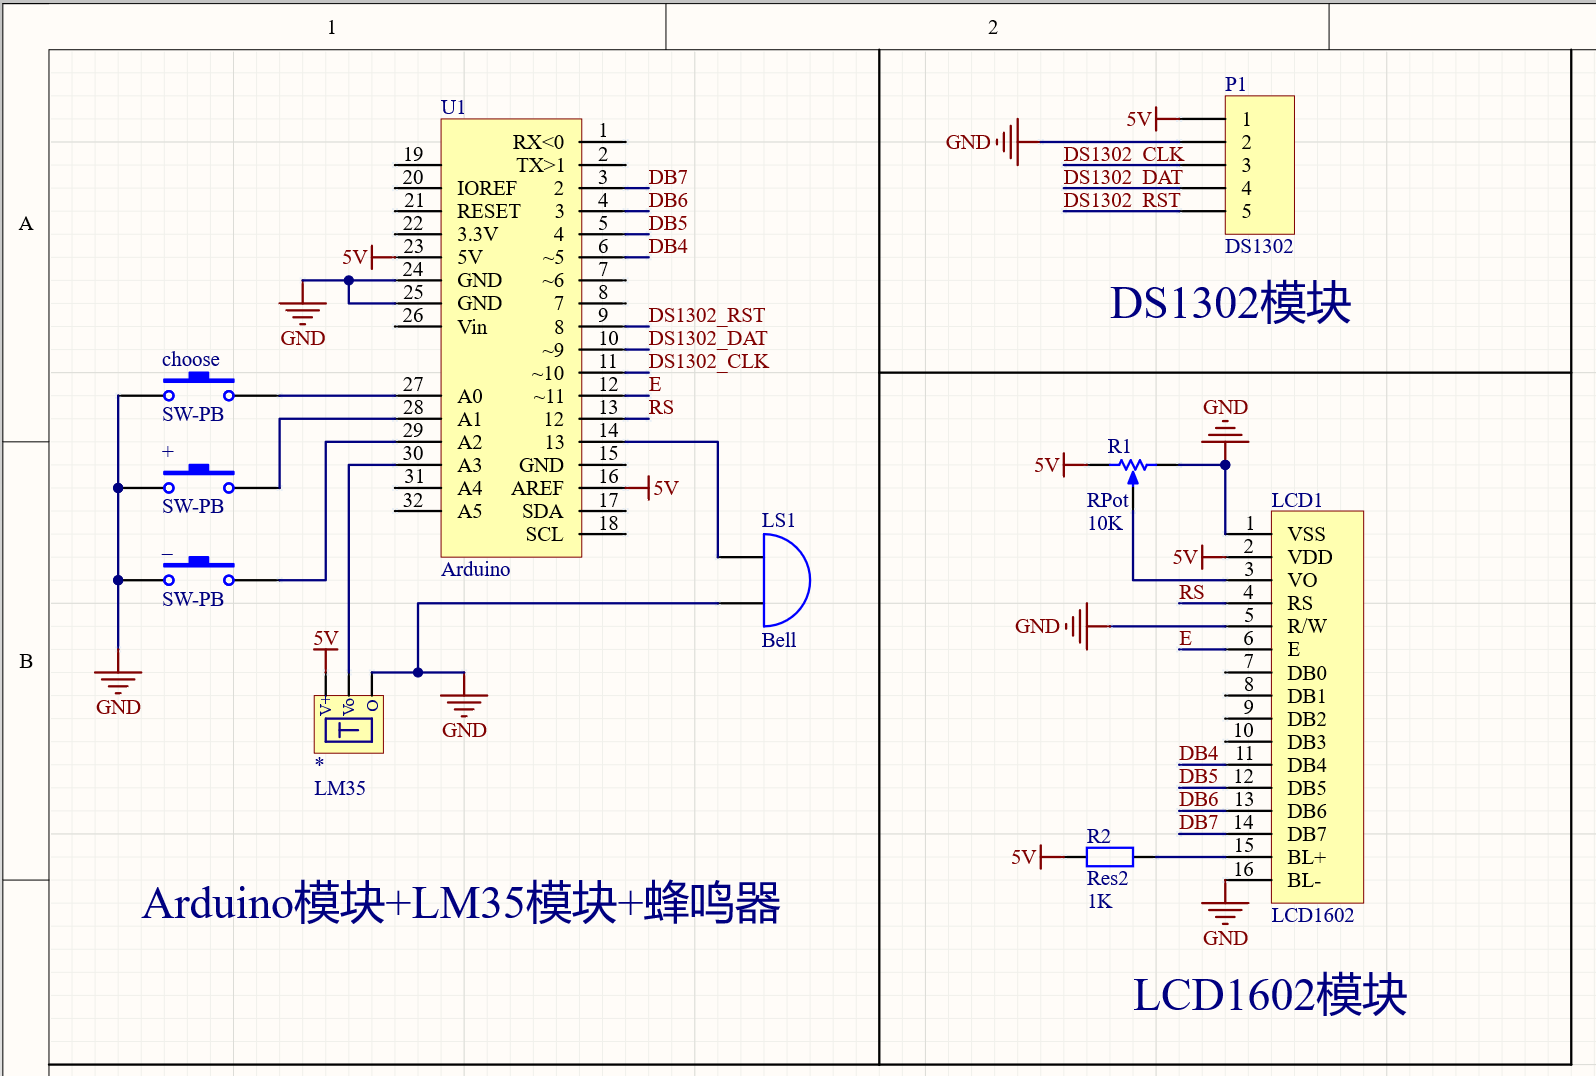
\includegraphics[width=0.6\textwidth]{figures/p2.png}
    \caption{原理图}
\end{figure}

\subsection{PCB图}
\begin{figure}[H]
    \centering
    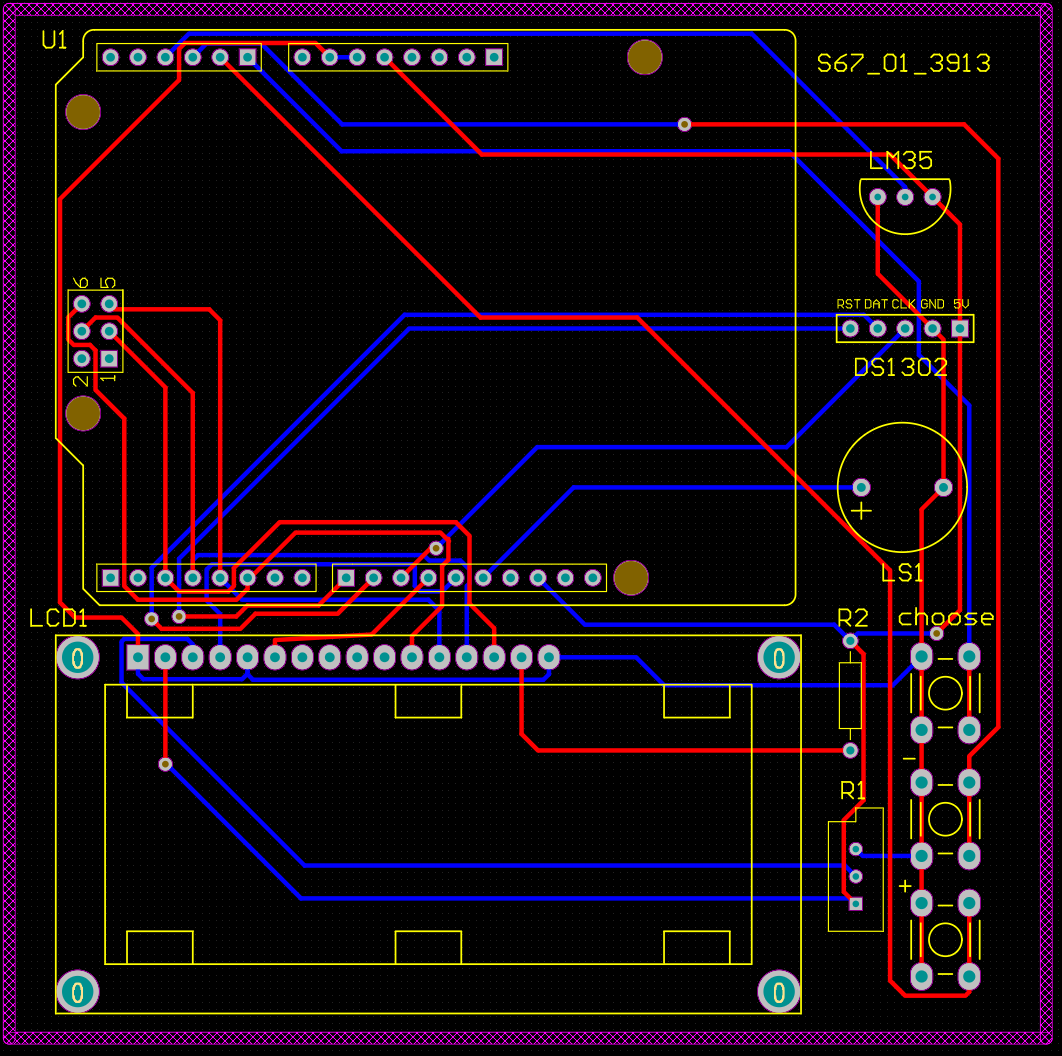
\includegraphics[width=0.6\textwidth]{figures/p3.png}
    \caption{PCB图}
\end{figure}
\clearpage
\section{实验设计总结}
通过参与本次原理图与PCB设计实验，我不仅在电子电路设计方面获得了显著的技能提升，还对从概念设计到实际实现的整体流程建立了更清晰、系统的认知。本次实验，我以Arduino UNO为核心平台，设计一个具备多功能的数字时钟。这项任务不仅充满挑战和趣味，也是一次对我已掌握知识的应用实践，同时也是对新技能、新技术的深入学习和探索。

在熟悉了Arduino编程环境之后，我专注于验证DS1302实时时钟模块和LCD1602液晶显示屏的有效性。这些硬件组件的连接并不仅仅是简单的物理操作，更重要的是确保它们在软件层面能够协同工作。这一过程要求我深入了解各模块的通信协议（如I²C或SPI）、电源需求以及显示控制逻辑，从而提升了我对嵌入式系统整合能力的理解。

进入硬件设计与PCB布板阶段后，Altium Designer的强大功能为整个设计提供了可能。尽管这款软件起初因复杂的界面和繁多的功能令人望而生畏，但随着不断的学习与反复尝试，诸如分层结构、设计规则检查（DRC）等功能逐渐变得得心应手。在原理图设计过程中，我注重元器件选型与封装匹配，并考虑了信号完整性等关键因素；而在PCB布局与布线阶段，我也经历了多次优化与调整，以满足电气性能和制造可行性要求。

通过这一系列密集且细致的实践，我掌握了如何将抽象的电路原理转化为可实际加工和测试的PCB版图，并在过程中深刻理解了诸多设计原则的实际应用。这种经历不仅增强了我的工程实践能力，也为我今后在电子工程领域的专业发展奠定了坚实基础。未来，我将以更加系统化、专业化的视角应对各类电路设计挑战，不断提升自身的技术水平与创新能力。
\section{代码段}
在原来代码基础上，考虑添加一个省电模式，通过长按选择键进入或退出省电模式,当处于省电模式时，关闭一些功能如温度检测，并改变显示更新频率。
\begin{lstlisting}[language=C++, caption=Arduino数字时钟新增代码]

// 在文件顶部声明省电模式状态变量
boolean powerSaveMode = false;

// 修改 setup 函数初始化省电模式状态
void setup(){ 
    // 原有的 setup 代码...

    // 初始化省电模式为关闭
    powerSaveMode = false;
}

// 添加进入/退出省电模式的函数
void togglePowerSaveMode() {
    powerSaveMode = !powerSaveMode;
    if(powerSaveMode) {
        lcd.clear();
        lcd.print("Power Save On");
        delay(1000); // 给用户看到提示信息的时间
    } else {
        lcd.clear();
        lcd.print("Normal Mode");
        delay(1000);
    }
}

// 修改 loop 函数以适应省电模式
void loop() { 
    seconds = millis()/1000; // 获取单片机当前运行时间
    
    if(digitalRead(choose) == LOW) {
        delay(1000); // 检测长按选择键
        if(digitalRead(choose) == LOW) {
            togglePowerSaveMode();
        }
    }

    if(!powerSaveMode) {
        Display(); // 显示时间
        Set_Clock(); // 设置时间
        Set_Alarm(); // 设置闹钟
        Point_Time_Alarm(); // 正点蜂鸣
        Clock_Alarm(); // 闹钟时间蜂鸣
        GetTemperatures(); // 获取 LM35 温度
        Temperatures_Alarm(); // 超过指定温度报警
    } else {
        // 省电模式下仅显示时间，减少其他操作
        time();
        delay(60000); // 每分钟更新一次时间显示
    }

    // 将单片机的当前时间写到 DS1302 芯片中
    rtc.setTime(hour,minute,second);
    rtc.setDate(day,month,year);
}
\end{lstlisting}

\begin{lstlisting}[language=C++, caption=Arduino数字时钟代码]
    * LCD RS pin to digital pin 12
    * LCD Enable pin to digital pin 11
    * LCD D4 pin to digital pin 5* LCD D5 pin to digital pin 4* LCD D6 pin to digital pin 3* LCD D7 pin to digital pin 2* LCD R/W pin to ground* LCD VSS pin to ground* LCD VCC pin to 5V 
    36
    * */
    #include <DS1302.h>
    #include <LiquidCrystal.h> //LCD1602 显示头文件
    LiquidCrystal lcd(12, 11, 5, 4, 3, 2); 
    #define choose A0 //选择端口
    #define add A1 //加
    #define minus A2 //减
    #define Tone 13 //蜂鸣器端口
    uint8_t CE_PIN = 8; //DS1302 RST 端口
    uint8_t IO_PIN = 9; //DS1302 DAT 端口
    uint8_t SCLK_PIN = 10; //DS1302 CLK 端口
    DS1302 rtc(CE_PIN, IO_PIN, SCLK_PIN); //创建 DS1302 对象
    unsigned long seconds;int s = 0, m = 0, h = 0, d = 0, mon = 0, y = 0; //时间进位
    int second = 0, minute = 0, hour = 0, day = 0, month = 0, year = 0; //当前时间
    int SECOND = 0, MINUTE = 0, HOUR = 0, DAY = 0, MONTH = 0, YEAR = 0; //初始时间
    int chose = 0, alarm_choose = 0 ,ButtonDelay = 20, frequence = 2093;int alarm_hour = 7, alarm_minute = 30, alarm_second = 0; //闹钟时间
    float Temperatures, Temp_Alarm = 30 ; 
    
    /** 格式化输出 */
    void FormatDisplay(int col, int row,int num){
        lcd.setCursor(col, row); 
        if(num < 10) lcd.print("0");
        lcd.print(num); 
    }
    
    /** 计算时间 */
    void time() { 
        second = (SECOND + seconds) % 60; //计算秒
        m = (SECOND + seconds) / 60; //分钟进位
        FormatDisplay(6,1,second);
        minute = (MINUTE + m) % 60; //计算分钟
        h = (MINUTE + m) / 60; //小时进位
        FormatDisplay(3,1,minute); 
        hour = (HOUR + h) % 24; //计算小时
        d = (HOUR + h) / 24; //天数进位
        FormatDisplay(0,1,hour); 
        lcd.setCursor(2, 1); 
        lcd.print(":"); 
        lcd.setCursor(5, 1); lcd.print(":"); 
    }
    
    /** 根据年月计算当月天数 */
    int Days(int year, int month){
        int days = 0;
        if (month != 2){
            switch(month){
                case 1: case 3: case 5: case 7: case 8: case 10: case 12: days = 31; break;
                case 4: case 6: case 9: case 11: days = 30; break;
            }
        }else{ //闰年
            if(year % 4 == 0 && year % 100 != 0 || year % 400 == 0){
                days = 29; 
            } 
            else{
                days = 28; 
            } 
        } 
        return days; 
    }
    
    /** 计算当月天数 */ 
    void Day(){ 
        int days = Days(year,month);
        int days_up;
        if(month == 1){
            days_up = Days(year - 1, 12); 
        } 
        else{
            days_up = Days(year, month - 1);
        } 
        day = (DAY + d) % days;
        if(day == 0){
            day = days; 
        } 
        if((DAY + d) == days + 1 ){
            DAY -= days;
            mon++;
        }
        if((DAY + d) == 0){
            DAY += days_up;
            mon--;
        }
        FormatDisplay(8,0,day); 
    }
    
    /** 计算月份 */
    void Month(){ 
        month = (MONTH + mon) % 12;
        if(month == 0){
            month = 12;
        } 
        y = (MONTH + mon - 1) / 12;
        FormatDisplay(5,0,month); 
        lcd.setCursor(7, 0); 
        lcd.print('-'); 
    }
    
    /** 计算年份 */
    void Year(){ 
        year = ( YEAR + y ) % 9999;
        if(year == 0){
            year = 9999;
        } 
        lcd.setCursor(0, 0); 
        if(year < 1000){ 
            lcd.print("0"); 
        }
        if(year < 100){ 
            lcd.print("0"); 
        }
        if(year < 10){ 
            lcd.print("0"); 
        }
        lcd.print(year);
        lcd.setCursor(4, 0); 
        lcd.print('-'); 
    }
    
    /** 根据年月日计算星期几 */
    void Week(int y,int m, int d){ 
        if(m == 1){
            m = 13;
        }
        if(m == 2){
            m = 14;
        } 
        int week = (d+2*m+3*(m+1)/5+y+y/4-y/100+y/400)%7+1; 
        String weekstr = "";
        switch(week){
            case 1: weekstr = "Mon. "; break;
            case 2: weekstr = "Tues. "; break;
            case 3: weekstr = "Wed. "; break;
            case 4: weekstr = "Thur. "; break;
            case 5: weekstr = "Fri. "; break;
            case 6: weekstr = "Sat. "; break;
            case 7: weekstr = "Sun. "; break;
        } 
        lcd.setCursor(11, 0); 
        lcd.print(weekstr);
    }
    
    /** 显示时间、日期、星期 */
    void Display() { 
        time();
        Day(); 
        Month();
        Year();
        Week(year,month,day); 
    }
    
    /** 显示光标 */
    void DisplayCursor(int rol, int row) {
        lcd.setCursor(rol, row); 
        lcd.cursor();
        delay(100); 
        lcd.noCursor();
        delay(100); 
    }
    
    /** 设置初始时间 */
    void set(int y, int mon, int d, int h, int m, int s){
        YEAR = y;
        MONTH = mon;
        DAY = d; 
        HOUR = h;
        MINUTE = m;
        SECOND = s; 
    }
    
    /** 通过按键设置时间 */
    void Set_Time(int rol, int row, int &Time){
        DisplayCursor(rol, row); 
        if(digitalRead(add) == LOW){
            delay(ButtonDelay);
            if(digitalRead(add) == LOW){
                Time ++;
            } 
            Display(); 
        } 
        if(digitalRead(minus) == LOW){
            delay(ButtonDelay);
            if(digitalRead(minus) == LOW){
                Time --; 
            } 
            Display(); 
        }
    }
    
    /** 按键选择 */
    void Set_Clock(){
        if(digitalRead(choose)==LOW){ 
            lcd.setCursor(9, 1); 
            lcd.print("SetTime");
            while(1){ 
                if(digitalRead(choose) == LOW){
                    delay(ButtonDelay);
                    if(digitalRead(choose) ==LOW){
                        chose++; 
                    }
                } 
                seconds = millis()/1000; 
                Display(); 
                if(chose == 1){
                    Set_Time(1, 1, HOUR); //SetHour
                }else if(chose == 2){ 
                    Set_Time(4, 1, MINUTE); //SetMinute
                }else if(chose == 3){
                    Set_Time(7, 1, SECOND); //SetSecond
                }else if(chose == 4){
                    Set_Time(9, 0, DAY); //SetDay
                }else if(chose == 5){
                    Set_Time(6, 0, MONTH); // SetMonth
                }else if(chose == 6){ 
                    Set_Time(3, 0, YEAR); //SetYear
                }else if(chose >= 7) {
                    chose = 0; 
                    break;
                }
            }
            delay(150);//新增（2024）
        } 
    }
    
    /** 设置闹钟小时 */
    void Set_Alarm_Hour(){
        DisplayCursor(1, 1); 
        if(digitalRead(add) == LOW){
            delay(ButtonDelay);
            if(digitalRead(add) == LOW){
                alarm_hour ++;
                if(alarm_hour == 24){
                    alarm_hour = 0;
                } 
                FormatDisplay(0,1,alarm_hour); 
            }
        }
        if(digitalRead(minus) == LOW){
            delay(ButtonDelay);
            if(digitalRead(minus) == LOW){ 
                alarm_hour --;
                if(alarm_hour == -1){
                    alarm_hour = 23;
                } 
                FormatDisplay(0,1,alarm_hour); 
            }
        }
    }
    
    /** 设置闹钟分钟 */
    void Set_Alarm_Minute(){
        DisplayCursor(4, 1); 
        if(digitalRead(add) == LOW) {
            delay(ButtonDelay);
            if(digitalRead(add) == LOW){
                alarm_minute ++;
                if(alarm_minute == 60){
                    alarm_minute = 0;
                } 
                FormatDisplay(3,1,alarm_minute); 
            }
        }
        if(digitalRead(minus) == LOW){
            delay(ButtonDelay);
            if(digitalRead(minus) == LOW){ 
                alarm_minute --;
                if(alarm_minute == -1){
                    alarm_minute = 59;
                } 
                FormatDisplay(3,1,alarm_minute); 
            } 
        } 
    }
    
    /** 设置报警温度 */
    void Set_Alarm_Temp(){ 
        DisplayCursor(10, 1); 
        if(digitalRead(add) == LOW) {
            delay(ButtonDelay);
            if(digitalRead(add) == LOW){
                Temp_Alarm ++; 
            } 
        }
        if(digitalRead(minus) == LOW){
            delay(ButtonDelay);
            if(digitalRead(minus) == LOW){
                Temp_Alarm --; 
            } 
        }
    }
    
    /** 进入报警设置 */
    void Set_Alarm(){
        if(digitalRead(add) == LOW && digitalRead(minus) == LOW){
            alarm_hour = hour;
            alarm_minute = minute;
            //alarm_choose = 1;
            lcd.setCursor(0, 0); 
            lcd.print("set alarm "); 
            lcd.setCursor(6, 1); 
            lcd.print("00"); //闹钟秒数
            while(1){
                if(digitalRead(choose) == LOW){
                    delay(ButtonDelay);
                    if(digitalRead(choose) == LOW){
                        alarm_choose++; 
                    } 
                }
                lcd.setCursor(9, 1); 
                lcd.print(Temp_Alarm);
                lcd.setCursor(14, 1); 
                lcd.print((char)223); //显示 o 符号
                lcd.setCursor(15, 1); 
                lcd.print("C"); //显示字母 C 
                if(alarm_choose == 1){
                    Set_Alarm_Hour();
                }else if(alarm_choose == 2){
                    Set_Alarm_Minute(); 
                }else if(alarm_choose == 3){
                    Set_Alarm_Temp(); 
                }else if(alarm_choose >= 4){
                    alarm_choose = 0;
                    break;
                } 
            }
            delay(150);
        }
    } 
    
    /** 正点蜂鸣 */
    void Point_Time_Alarm(){
        if(minute == 0 && second == 0){
            tone(Tone,frequence); 
            delay(500);
            noTone(Tone); 
        } 
    }
    
    /** 闹钟 指定时间蜂鸣 */
    void Clock_Alarm(){
        if(hour == alarm_hour && minute == alarm_minute && second == alarm_second){
            tone(Tone,frequence); 
            delay(5000);
            noTone(Tone); 
        }
    } 
    
    /** 获取 LM35 温度 */
    void GetTemperatures(){
        long a = analogRead(A3); // Get temperatures
        Temperatures = 500.0*a/1023.0;
        lcd.setCursor(9, 1) ; 
        lcd.print(Temperatures); //获取温度
        lcd.setCursor(14, 1); 
        lcd.print((char)223); //显示 o 符号
        lcd.setCursor(15, 1); 
        lcd.print("C"); //显示字母 C 
    }
    
    /** 超过指定温度报警 */
    void Temperatures_Alarm(){
        if(Temperatures >= Temp_Alarm){
            tone(Tone,frequence); 
            delay(500);
            noTone(Tone); 
        }
    }
    
    void setup(){ 
        for(int i = 2;i <= 13; i++){
            pinMode(i,OUTPUT); 
        } 
        digitalWrite(add, HIGH);
        digitalWrite(minus, HIGH);
        digitalWrite(choose, HIGH); 
        lcd.begin(16, 2); //初始化 LCD1602 
        //读取 DS1302 芯片的时间
        rtc.writeProtect(false); // 关闭 DS1302 芯片写保护
        rtc.halt(false); 
        //为 true 时 DS1302 暂停
        Time t;
        t=rtc.getTime();
        set(t.year,t.mon,t.date,t.hour,t.min,t.sec); //设置 DS1302 芯片初始时间
        // Time t;
        // t.hour=10;t.min=47;t.sec=59;
        // t.year=2025;t.mon=2;t.date=12;
        // rtc.setTime(t.hour,t.min,t.sec); //设置 DS1302 芯片初始时间
        // rtc.setDate(t.year,t.mon,t.date);
        // set(t.year,t.mon,t.date,t.hour,t.min,t.sec);
    }
    
    void loop() { 
        seconds = millis()/1000; //获取单片机当前运行时间
        Display(); //显示时间
        Set_Clock(); //设置时间
        Set_Alarm(); //设置闹钟
        Point_Time_Alarm(); //正点蜂鸣
        Clock_Alarm(); //闹钟时间蜂鸣
        GetTemperatures(); //获取 LM35 温度
        Temperatures_Alarm(); //超过指定温度报警
        //将单片机的当前时间写到 DS1302 芯片中
        rtc.setTime(hour,minute,second);
        rtc.setDate(day,month,year);
    }
\end{lstlisting}
\end{document}
